\documentclass{beamer}

\mode<presentation> {

% The Beamer class comes with a number of default slide themes
% which change the colors and layouts of slides. Below this is a list
% of all the themes, uncomment each in turn to see what they look like.

%\usetheme{default}
%\usetheme{AnnArbor}
%\usetheme{Antibes}
%\usetheme{Bergen}
%\usetheme{Berkeley}
%\usetheme{Berlin}
%\usetheme{Boadilla}
%\usetheme{CambridgeUS}
%\usetheme{Copenhagen}
%\usetheme{Darmstadt}
%\usetheme{Dresden}
%\usetheme{Frankfurt}
%\usetheme{Goettingen}
%\usetheme{Hannover}
%\usetheme{Ilmenau}
%\usetheme{JuanLesPins}
%\usetheme{Luebeck}
\usetheme{Madrid}

\usepackage{hyperref}
\usepackage{amsmath}
\usepackage{amsthm}
\usepackage{amsfonts}
\usepackage{amssymb}
\newtheorem{definicija}{Definicija}
% naložite dodatne pakete, ki jih potrebujete
\usepackage{units}        % fizikalne enote kot \unit[12]{kg} s polovico nedeljivega presledka, glej primer v kodi
\usepackage{graphicx}     % za slike
\usepackage{graphicx}
\usepackage{subcaption}
\usepackage[utf8]{inputenc}
\usepackage[T1]{fontenc}
\usepackage{lmodern}
\usepackage{amsmath}
\usepackage{amsthm}
\usepackage{amsfonts}
\usepackage{amssymb}
\usepackage{enumitem}
\usepackage{commath}
\usepackage{mathtools}
\usepackage{adjustbox}
\usepackage{setspace}
\usepackage{bigints}
\usepackage{hyperref}
\usepackage{caption}
\usepackage{mathrsfs}


% VEČ ZANIMIVIH PAKETOV
% \usepackage{array}      % več možnosti za tabele
% \usepackage[list=true,listformat=simple]{subcaption}  % več kot ena slika na figure, omogoči slika 1a, slika 1b
% \usepackage[all]{xy}    % diagrami
% \usepackage{doi}        % za clickable DOI entrye v bibliografiji
 \usepackage{enumerate}     % več možnosti za sezname

% Za barvanje source kode
% \usepackage{minted}
% \renewcommand\listingscaption{Program}

% Za pisanje psevdokode
% \usepackage{algpseudocode}  % za psevdokodo
% \usepackage{algorithm}
% \floatname{algorithm}{Algoritem}
% \renewcommand{\listalgorithmname}{Kazalo algoritmov}

% deklarirajte vse matematične operatorje, da jih bo LaTeX pravilno stavil
% \DeclareMathOperator{\...}{...}

% vstavite svoje definicije ...
\newcommand{\R}{\mathbb R}
\newcommand{\N}{\mathbb N}
\newcommand{\Z}{\mathbb Z}
\newcommand{\bd}{\textbf}
% Lahko se zgodi, da je ukaz \C definiral že paket hyperref,
% zato dobite napako: Command \C already defined.
% V tem primeru namesto ukaza \newcommand uporabite \renewcommand
\newcommand{\C}{\mathbb C}
\newcommand{\Q}{\mathbb Q}


% As well as themes, the Beamer class has a number of color themes
% for any slide theme. Uncomment each of these in turn to see how it
% changes the colors of your current slide theme.

%\usecolortheme{albatross}
%\usecolortheme{beaver}
%\usecolortheme{beetle}
%\usecolortheme{crane}
%\usecolortheme{dolphin}
%\usecolortheme{dove}
%\usecolortheme{fly}
%\usecolortheme{lily}
%\usecolortheme{orchid}
%\usecolortheme{rose}
%\usecolortheme{seagull}
%\usecolortheme{seahorse}
%\usecolortheme{whale}
%\usecolortheme{wolverine}

%\setbeamertemplate{footline} % To remove the footer line in all slides uncomment this line
%\setbeamertemplate{footline}[page number] % To replace the footer line in all slides with a simple slide count uncomment this line

%\setbeamertemplate{navigation symbols}{} % To remove the navigation symbols from the bottom of all slides uncomment this line
}

%----------------------------------------------------------------------------------------
%    TITLE PAGE
%----------------------------------------------------------------------------------------

\title[Long title]{Turbulence in Large eddy simulacije} % The short title appears at the bottom of every slide, the full title is only on the title page

\author{Uroš Kosmač} % Your name
\institute[FMF] % Your institution as it will appear on the bottom of every slide, may be shorthand to save space
{
Fakulteta za matematiko in fiziko\\ % Your institution for the title page
\textit{Mentor: prof. dr. Emil Žagar}\\ % Your email address
\textit{Somentor: dr. Peter Smerkol} % Your email address
}
\date{\today} % Date, can be changed to a custom date

%\hypersetup{pdfpagemode=FullScreen}

\begin{document}

\begin{frame}
\titlepage % Print the title page as the first slide
\end{frame}

    

\begin{frame}
\frametitle{Uvod}
Kaj je turbulenca? \\
\pause
\begin{itemize}
    \item[\Large$\cdot$] Kaotičnost
    \pause
    \item[\Large$\cdot$] Vrtinci 
    \begin{figure}[h!]
        \centering
        \begin{subfigure}{.5\textwidth}
          \centering
          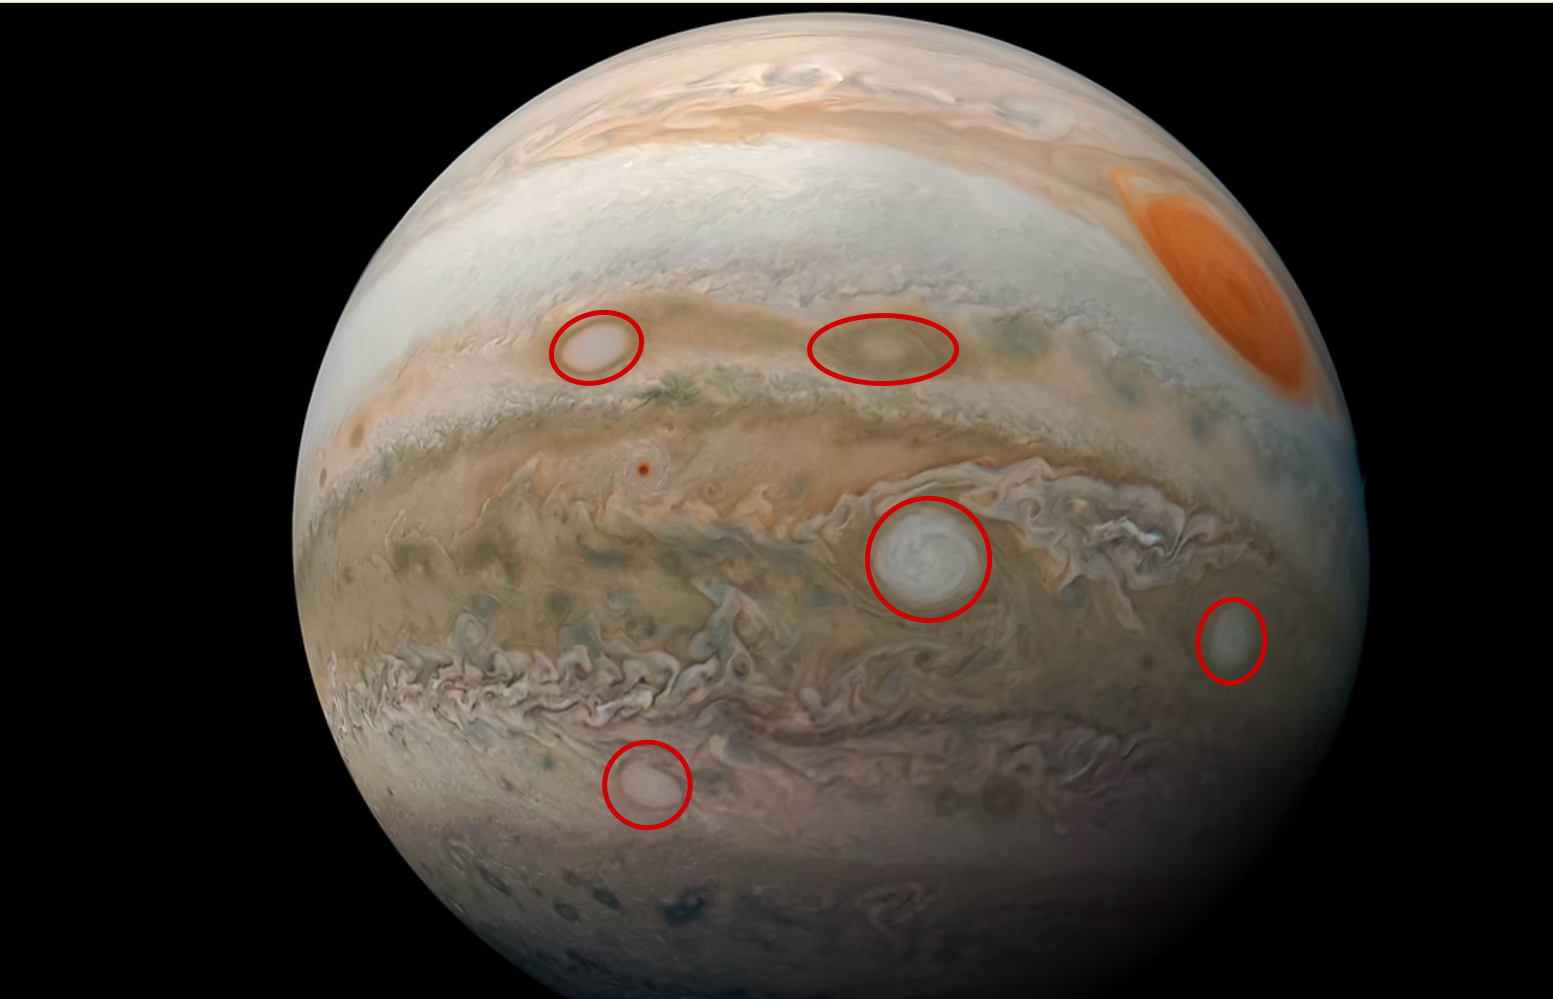
\includegraphics[width=0.95\linewidth]{slike/vrtinci.jpeg}
          %\caption{A subfigure}
          %\label{fig:sub1}
        \end{subfigure}%
        \begin{subfigure}{.5\textwidth}
          \centering
          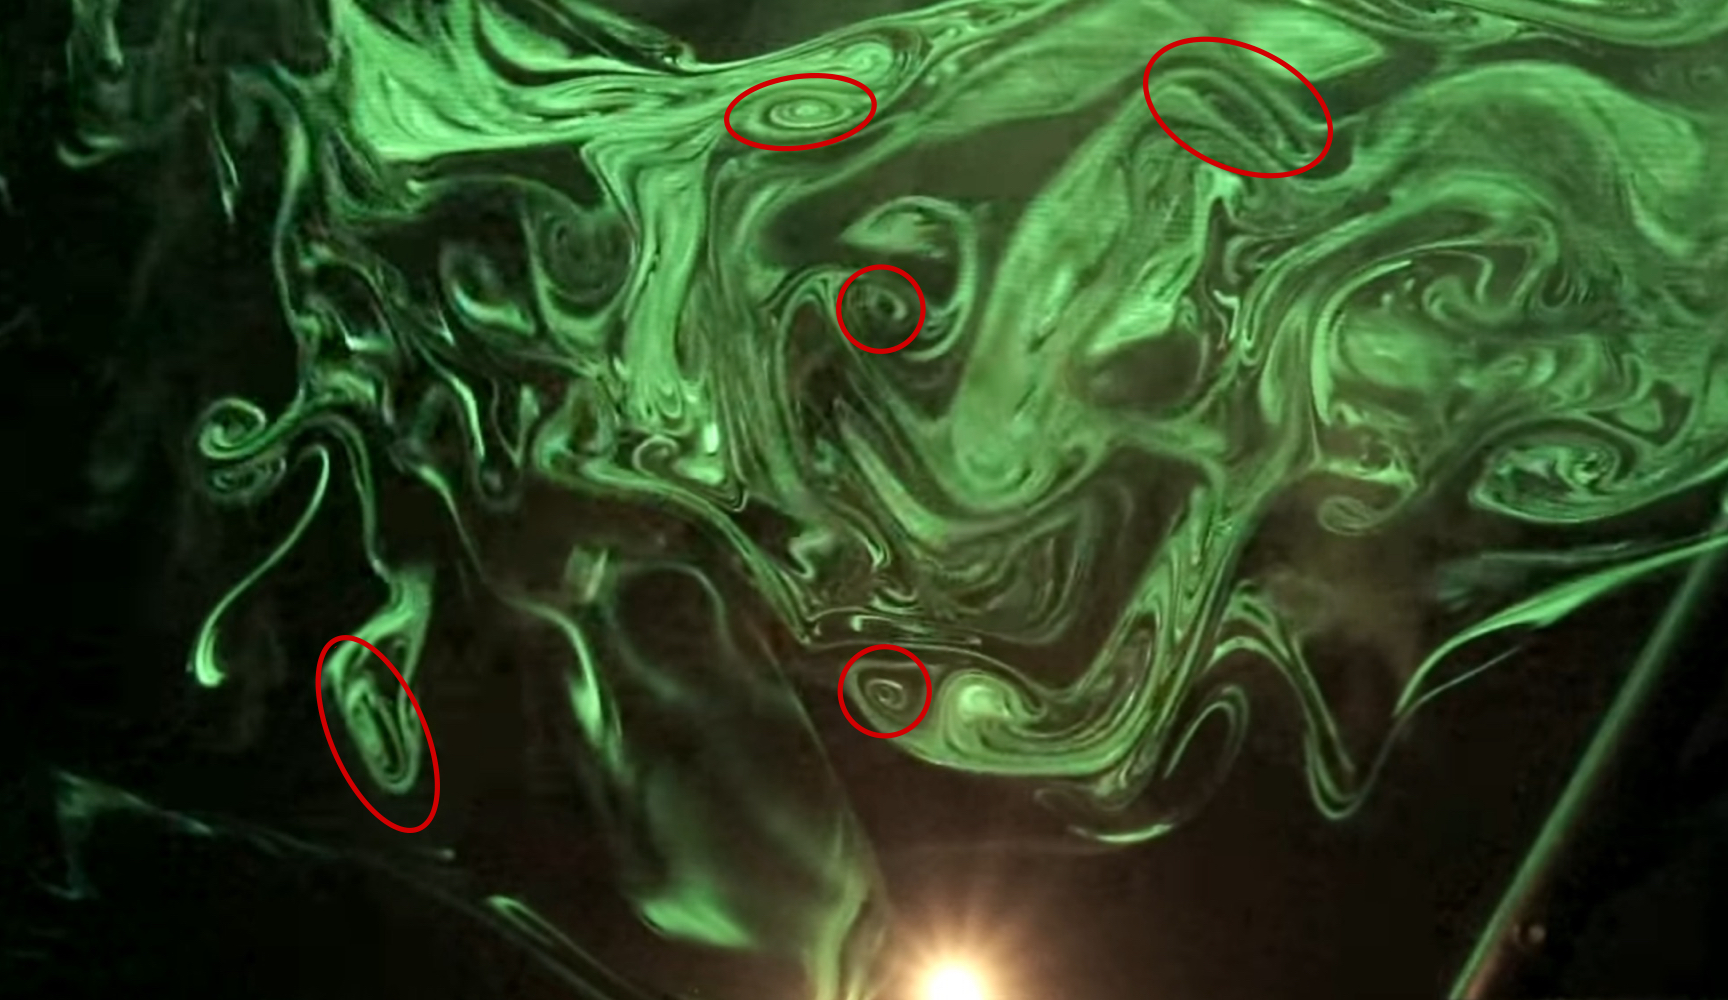
\includegraphics[height=4.58cm, width=0.95\linewidth]{slike/vrtinci2.jpeg}
          %\caption{A subfigure}
          %\label{fig:sub2}
        \end{subfigure}
        \end{figure}
\end{itemize}
\end{frame}
\begin{frame}
\begin{itemize}
    \item[\Large$\cdot$] Difuzivnost
    \begin{figure}[h!]
        \centering
      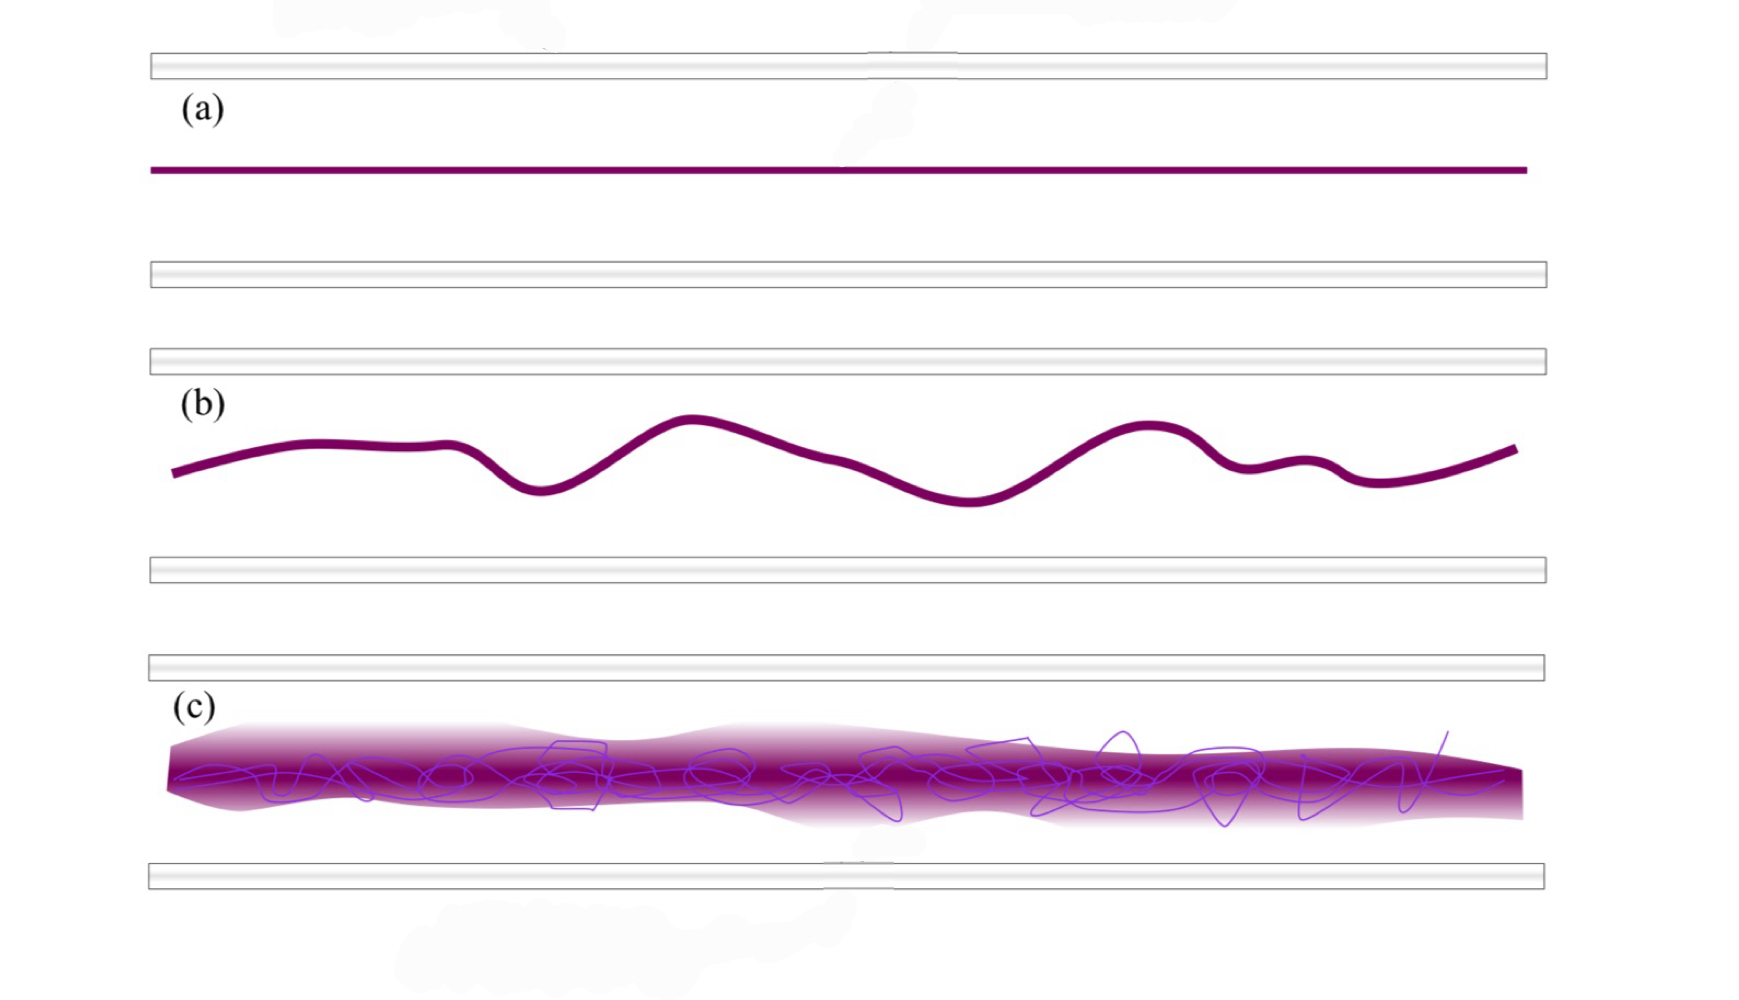
\includegraphics[scale=0.19]{slike/difus.jpeg}
      \end{figure}
\end{itemize}
\end{frame}
\begin{frame}
\begin{itemize}
    \item[\Large$\cdot$] Reynoldsovo število
    \begin{figure}[h]
        \centering
      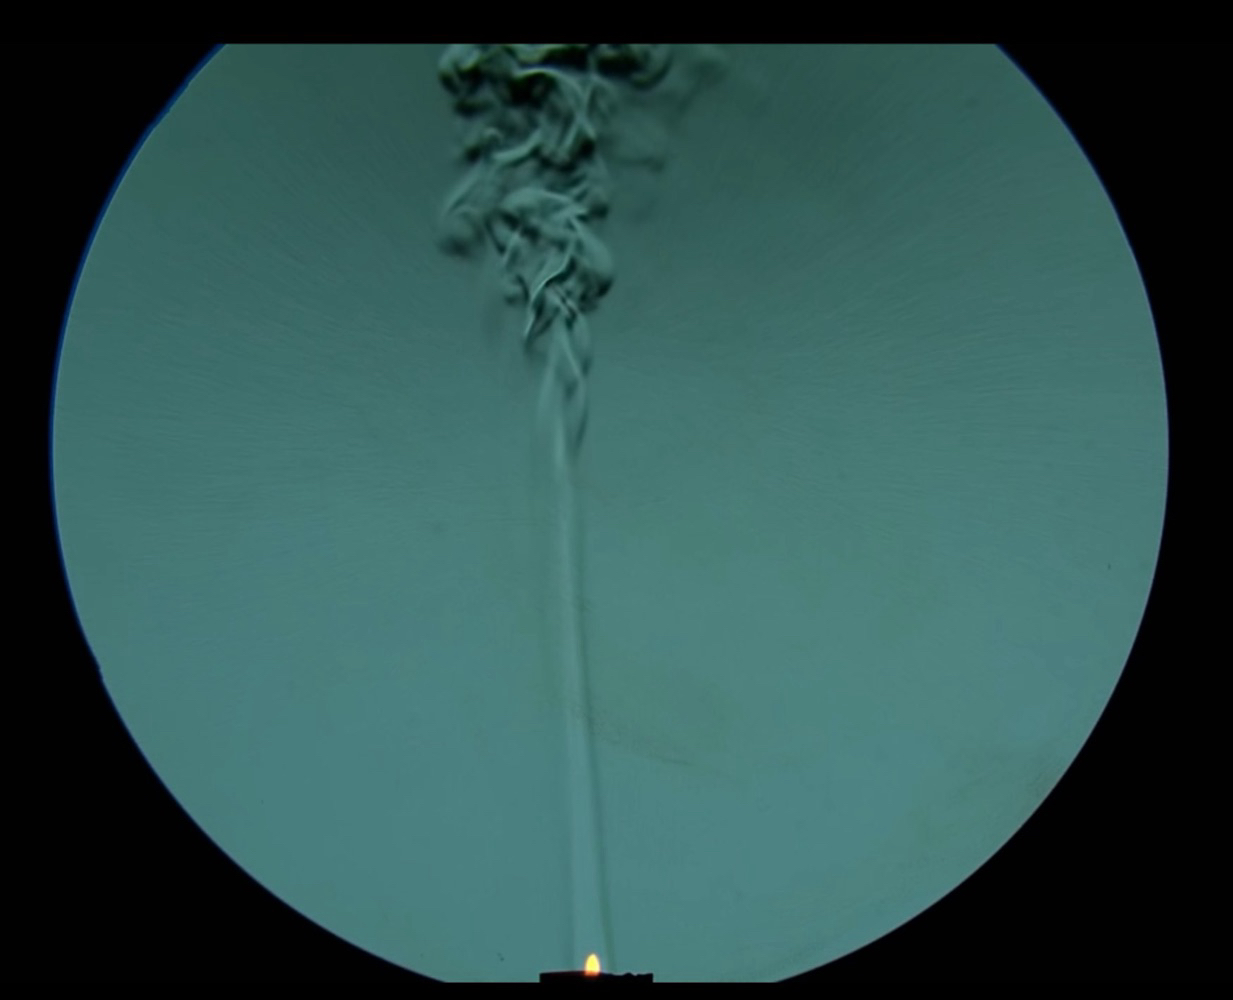
\includegraphics[scale=0.19]{slike/Reynolds.jpeg}
      \end{figure}
    \pause
    \item[\Large$\cdot$] Disipativnost
\end{itemize}
\end{frame}

\begin{frame}
    \frametitle{Dva pristopa}
Tok lahko obravnavamo na dva različna načina. Naj bo $\Omega \subset \mathbb{R}^3$:
\begin{itemize}
    \pause
\item Eulerjev pristop: tok je preslikava
\begin{align*}
    \textbf{u}: \Omega \times \R^+ &\rightarrow \R^3 \\
    (\bd{x},t) \mapsto&\,\, \textbf{u}(\bd{x},t).
\end{align*}
\pause
\item Lagrangev pristop: dana je trajektorija 
\begin{align*}
    \bd{X}: \R^+& \rightarrow \R^3 \\
    t \mapsto&\,\, \bd{X}(t; \bd{x}_0),
\end{align*}
za začetno točko $\bd{x}_0$ in $\bd{X}(t_0; \bd{x}_0) = \bd{x}_0$
\end{itemize}
\end{frame}

\begin{frame}
Relacija med njima: 
\begin{align*}
    U(t;\bd{x}_0) = \frac{\dif X}{\dif t}&(t; \bd{x}_0) = \bd{u}(X(t; \bd{x}_0), t),
\end{align*}
\pause 
\begin{definicija}
    Naj bo $\Omega \subset \R^n$ in $\bd{v}: \Omega\times \R^+ \rightarrow \R^n$ vektorsko polje. Diferencialni operator 
    $\frac{D}{D t}: C^1(\Omega \times \R^+, \R^n) \rightarrow C^0(\Omega \times \R^+, \R^n)$ dan s predpisom
    \begin{equation}
        \frac{D \bd{u}}{Dt} = \Big(\frac{\partial}{\partial t} + \bd{v} \cdot \nabla_{\bd{x}}\Big) \bd{u} = \frac{\partial \bd{u}}{\partial t} + (v\cdot \nabla_x) u
    \end{equation}
\end{definicija}
\pause
\begin{equation}
    \frac{\dif}{\dif t} U(t; \bd{x}_0) = \Big(\frac{D \bd{u}}{Dt}(\bd{x}, t) \Big)_{\bd{x} = X(t; \bd{x}_0)},
\end{equation}
\end{frame}


\begin{frame}
\frametitle{Ohraniteni zakoni}
\begin{itemize}
    \pause
    \item \textbf{Ohranitev mase}:
    \begin{equation}
        \frac{\partial \rho}{\partial t} + \nabla \cdot (\rho \bd{u}) = 0.
    \end{equation}
    \pause
    \item \textbf{Ohranitev gibalne količine}:
    \item 
    \begin{equation}
    \rho \frac{\partial \bd{u}}{\partial t} + \rho(\bd{u}\cdot \nabla_x) u = - \nabla p + \mu \nabla^2 \bd{u} + \bd{f},
    \end{equation}
    \pause
    \item \textbf{Ohranitev vrtinčenja}:
    \begin{equation}
    \frac{\partial \bd{$\omega$}}{\partial t} + (\bd{u}\cdot \nabla)\bd{$\omega$} = (\bd{$\omega$} \cdot \nabla)\bd{u}+ \nu \nabla^2 \bd{$\omega$} + \nabla \times \bd{f}
    \end{equation}
    \pause
    \item \textbf{Ohranitev skalarja}:
    \begin{equation}
        \frac{\partial c}{\partial t} + \bd{u}\cdot\nabla c = \gamma \nabla^2 c.
    \end{equation}        
\end{itemize}
\end{frame}

\begin{frame}
\frametitle{Reynoldsovo število}
\pause
Enačbo za gibalno količino, preko transformacij 
$$
\tilde{\bd{u}} = \frac{\bd{u}}{U}, \quad \tilde{p} = \frac{p}{\rho U^2}, \quad \tilde{\bd{f}} = \bd{f}\frac{\rho L}{U^2},
\quad \frac{\partial}{\partial \tilde{t}} = \frac{L}{U} \frac{\partial}{\partial t}, \quad 
\tilde{\nabla} = L\nabla
$$
za $L, U > 0$ prevedemo na \bd{brezdimenzijsko Navier-Stokesovo enačbo}:
$$
\frac{D\tilde{u}}{D \tilde{t}} = \frac{\partial \tilde{\bd{u}}}{\partial \tilde{t}} + 
(\tilde{\bd{u}} \cdot \tilde{\nabla}) \tilde{\bd{u}} = - \tilde{\nabla} \tilde{p}
+ \underbrace{\frac{\mu}{\rho UL}}_{\frac{1}{Re}} \tilde{\nabla}^2 \tilde{\bd{u}} + \tilde{\bd{f}}
$$
\end{frame}

\begin{frame}
\frametitle{Reynoldsovo število}
Alternativna tranformacija, nam da:
\begin{equation*}
    Re\frac{D\tilde{\bd{u}}}{D \tilde{t}} =  - \tilde{\nabla} \tilde{p}
    + \tilde{\nabla}^2 \tilde{\bd{u}} + \tilde{f}.
\end{equation*}
Posledica: \href{https://www.youtube.com/watch?v=h1DnrWEOWeg&feature=youtu.be}{Časovna neodvisnost}
\end{frame}

\begin{frame}
\frametitle{Disipativnost}
Naj bo $\bd{f} = 0$ in predpostavimo $\bd{u}_{|_{\partial\Omega}} = 0$. 
\pause
Iz Navier-Stokesovih enačb izpeljemo:
\[
\frac{\partial}{\partial t}\int_\Omega \frac{1}{2} |\bd{u}|^2 \dif V = - \nu\int_\Omega |\nabla \bd{u}|^2 \dif V.
\]
\pause
Če $\bd{f} \neq 0$ in $\frac{\partial}{\partial t} |\bd{u}|^2 = 0$
dobimo 
\pause
\[
 \nu\int_\Omega |\nabla \bd{u}|^2 \dif V = \int_\Omega \bd{u}\cdot \bd{f} \dif V.
\]
Disipativnost "=" moč dela zunanjih sil.
\end{frame}


\begin{frame}
\frametitle{LES}
\pause
Posledica disipativnosti, nam domeno/območje razdeli na 
tri dele:
\begin{itemize}
\item[\Large$\cdot$] Energijsko bogato območje
\item[\Large$\cdot$] Inercijsko območje 
\item[\Large$\cdot$] Disipativno območje
\end{itemize}
\pause
LES
\begin{itemize}
    \item[\Large$\cdot$] Filtracija in filtrirane enačbe
    \pause
    \begin{align*} 
        \frac{\partial \overline{U}_j}{\partial t} + \frac{\partial \overline{U_i}\, \overline{U_j}}{\partial x_i} = -\frac{1}{\rho} \frac{\partial \overline{P}}{\partial x_j} 
- \frac{\partial \tau_{ij}^\text{anizo}}{\partial x_i}+ \nu \frac{\partial^2 \overline{U}_j}{\partial x_i \partial x_i} + \overline{f}_j,
    \end{align*}
    \pause
    \item[\Large$\cdot$] Problem zaprtja.
\end{itemize}
\end{frame}

\end{document}